\documentclass[conference]{IEEEtran}
% \IEEEoverridecommandlockouts
% The preceding line is only needed to identify funding in the first footnote. If that is unneeded, please comment it out.
\usepackage{cite}
\usepackage{amsmath,amssymb,amsfonts}
\usepackage{algorithmic}
\usepackage{graphicx}
\usepackage{textcomp}
\usepackage{xcolor}
\def\BibTeX{{\rm B\kern-.05em{\sc i\kern-.025em b}\kern-.08em
    T\kern-.1667em\lower.7ex\hbox{E}\kern-.125emX}}
\begin{document}

\title{Glycemic Increment: Individualized Medicine for Diabetics*\\
}

\author{\IEEEauthorblockN{1\textsuperscript{st} Jennifer Balasi}
\IEEEauthorblockA{\textit{iSchool} \\
\textit{Syracuse University}\\
Syracuse, NY, USA\\
balasij@gmail.com}
\and
\IEEEauthorblockN{2\textsuperscript{nd} La Monte Henry Piggy Yarroll}
\IEEEauthorblockA{\textit{iSchool} \\
\textit{Syracuse University}\\
Syracuse, NY, USA\\
ORCID 0009-0006-3073-6352}
}
\maketitle

\begin{abstract}
Glycemic Increment is a new metric for diabetics to estimate the glycemic effect of meals they eat regularly. It is based on a log of meals with blood sugar measurements from a Continuous Glucose Monitor.
\end{abstract}

\begin{IEEEkeywords}
diabetes, biomedical measurements, medical expert system
\end{IEEEkeywords}

\section{Introduction}
Diabetes is a common disease in the US. In 2021 38.4 million people of all ages—or 11.6\% of the U.S. population—had diabetes \cite{CDC_2024}. 97.6 million people aged 18 years or older had prediabetes (38.0\% of the adult U.S. population).

One of the first recommendations for people with prediabetes is lifestyle changes. People are encouraged to lose weight, exercise more, and restrict their intake of carbohydrates \cite{CDC_2024b}. Easily digested carbohydrates lead to elevated blood sugar, the core diagnostic trait of both type I and type II diabetes.

A core pillar of treatment is the regular monitoring of blood sugar. Regular monitoring has been found to reduce instances of hyperglycemia (high blood sugar), and hypoglycemia (low blood sugar due to insulin spikes).

In 1962, Leland Clark and Ann Lyons from Cincinnati Children's Hospital developed the sensor that led to the glucometer, which enabled home blood glucose monitoring (HBGM) \cite{Clark_1962}. A glucometer measures blood sugar by placing a drop of blood on a disposable sensor. Using a glucometer to monitor blood sugar requires high discipline, especially in insulin-dependent diabetes (type I and advanced type II).

Since the FDA approved the first continuous glucose monitor (CGM) in 1999 \cite{Reddy_2023}, there is a more convenient solution. A CGM is worn continuously for an extended period and provides automatic readings at a high frequency (typically every 5 minutes).

The apps associated with CGMs typically allow the user to record significant events such as meals or insulin doses. These meal logs are the basis for the new metric, Glycemic Increment.

\section{Metrics}

\subsection{Blood Glucose and HbA1c}

Blood glucose is measured in mg/dL. It is the primary metric generated by a CGM. See Figure \ref{fig:glucose_chart} for typical values.

Hemoglobin A1c (HbA1c) shows average blood sugar levels over the past 2-3 months expressed as a percentage. A CGM app can calculate an equivalent metric, Glucose Mangement Indicator (GMI), from continuous glucose values. HbA1c is often used to diagnose prediabetes or diabetes.

\begin{figure}[h]
    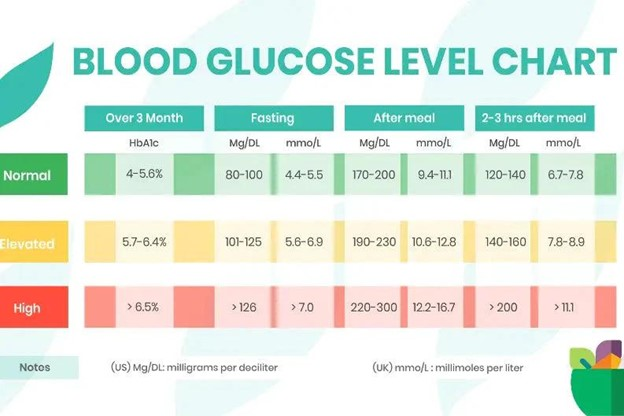
\includegraphics[width=0.5\textwidth]{images/Normal-Blood-Sugar-Levels-Chart.jpg}
    \label{fig:glucose_chart}
    \caption{Blood Glucose levels \protect\cite{Agarwal_2025}}
\end{figure}

\subsection{Glycemic Index GI}

An important innovation in relating foods to blood glucose was the introduction of Glycemic Index by \cite{Jenkins_1981}. Glycemic Index (GI) estimates how quickly a standard amount of carbohydrates (50g) is absorbed by the body from a specific food. It attempts to measure how quickly a food is absorbed. Measurements require the test subject to fast before eating the food. The amount of food varies according to its carbohydrate content. Blood glucose is then integrated over the next 2 hours. The resulting value is standardized against 50g of pure glucose, yielding a number from 0 (no effect on blood sugar) to 100 (same effect as pure glucose). There are some foods that have GI ratings higher than 100.

\subsection(Glycemic Load GL}

One limitation of GI is that it is difficult to translate into expectations for a given meal. Salmerón et. al. introduced the concept of Glycemic Load (GL) \cite{Salmeron_1997}, which improves upon GI by accounting for the amount of carbohydrates in a 100g serving of the food. In theory, this allows one to calculate a summary metric for any given meal to estimate the effects on blood sugar. In practice, it is a lot of work to weigh each food, look up its GL and then build a GL estimate for the meal. It can be very difficult to find the GL for certain foods. GI and GL also vary when certain foods are mixed.

\subsection{Glycemic Increment G+}

With the availability of CGM data, it becomes practical to directly estimate the glycemic effects of meals eaten by the patient. Actual measurements of typical meals can lead to actionable insights into diet.

This paper introduces the concept of Glycemic Increment (G+). G+ directly estimates the blood sugar consequences of particular foods and composite meals. It provides an individualized model of each patient's response to particular foods. The inputs to the model are just a list of foods in a particular meal. The output is a number that directly estimates an increase or decrease in blood sugar over a reasonable period. The model is built without requiring a fasting state or precise measurements of foods. It relies on the "typical serving" used by the patient.

Figure \ref{fig:gplus_illustrated} shows how G+ is calculated. The left of the chart represents the start of a meal. The duration of the chart represents the measurement period. The values in blue are the integration of blood glucose values over the measurement period. The orange area, set at the initial blood glucose level, is subtracted from the blue. The difference is divided by the number of hours in the measurement period. The resulting unit is mg-hours/dL.

Standardization to 1 hour allows for the comparison of G+ from different measurement intervals.

Using the starting blood glucose makes it unnecessary for the patient to be fasting.

Note that if blood glucose falls significantly below the starting glucose, G+ can yield a negative value. This can happen when a food triggers a rapid insulinic response, causing blood sugar to drop rapidly. For this reason, both very positive and very negative G+ values should be interpreted as a strong glycemic response.

It is not clear whether the low glycemic response is G+ values near zero or G+ values near the mean. Without further examination, the present work assumes the former.

\begin{figure}[h]
    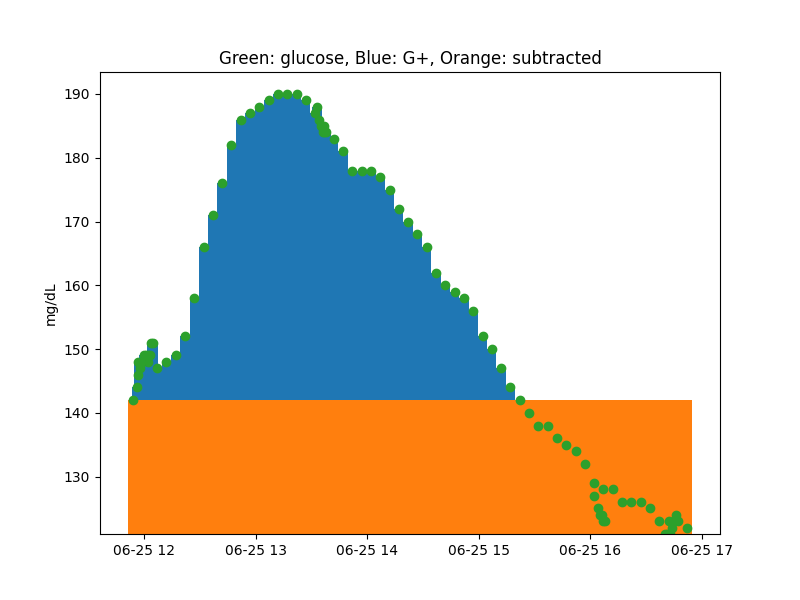
\includegraphics[width=0.5\textwidth]{images/gplus_illustrated.png}
    \label{fig:gplus_illustrated}
    \caption{Glycemic Increment}
\end{figure}

\section{Prepare Your Paper Before Styling}
Before you begin to format your paper, first write and save the content as a 
separate text file. Complete all content and organizational editing before 
formatting. Please note sections \ref{AA}--\ref{SCM} below for more information on 
proofreading, spelling and grammar.

Keep your text and graphic files separate until after the text has been 
formatted and styled. Do not number text heads---{\LaTeX} will do that 
for you.

\subsection{Abbreviations and Acronyms}\label{AA}
Define abbreviations and acronyms the first time they are used in the text, 
even after they have been defined in the abstract. Abbreviations such as 
IEEE, SI, MKS, CGS, ac, dc, and rms do not have to be defined. Do not use 
abbreviations in the title or heads unless they are unavoidable.

\subsection{Units}
\begin{itemize}
\item Use either SI (MKS) or CGS as primary units. (SI units are encouraged.) English units may be used as secondary units (in parentheses). An exception would be the use of English units as identifiers in trade, such as ``3.5-inch disk drive''.
\item Avoid combining SI and CGS units, such as current in amperes and magnetic field in oersteds. This often leads to confusion because equations do not balance dimensionally. If you must use mixed units, clearly state the units for each quantity that you use in an equation.
\item Do not mix complete spellings and abbreviations of units: ``Wb/m\textsuperscript{2}'' or ``webers per square meter'', not ``webers/m\textsuperscript{2}''. Spell out units when they appear in text: ``. . . a few henries'', not ``. . . a few H''.
\item Use a zero before decimal points: ``0.25'', not ``.25''. Use ``cm\textsuperscript{3}'', not ``cc''.)
\end{itemize}

\subsection{Equations}
Number equations consecutively. To make your 
equations more compact, you may use the solidus (~/~), the exp function, or 
appropriate exponents. Italicize Roman symbols for quantities and variables, 
but not Greek symbols. Use a long dash rather than a hyphen for a minus 
sign. Punctuate equations with commas or periods when they are part of a 
sentence, as in:
\begin{equation}
a+b=\gamma\label{eq}
\end{equation}

Be sure that the 
symbols in your equation have been defined before or immediately following 
the equation. Use ``\eqref{eq}'', not ``Eq.~\eqref{eq}'' or ``equation \eqref{eq}'', except at 
the beginning of a sentence: ``Equation \eqref{eq} is . . .''

\subsection{\LaTeX-Specific Advice}

Please use ``soft'' (e.g., \verb|\eqref{Eq}|) cross references instead
of ``hard'' references (e.g., \verb|(1)|). That will make it possible
to combine sections, add equations, or change the order of figures or
citations without having to go through the file line by line.

Please don't use the \verb|{eqnarray}| equation environment. Use
\verb|{align}| or \verb|{IEEEeqnarray}| instead. The \verb|{eqnarray}|
environment leaves unsightly spaces around relation symbols.

Please note that the \verb|{subequations}| environment in {\LaTeX}
will increment the main equation counter even when there are no
equation numbers displayed. If you forget that, you might write an
article in which the equation numbers skip from (17) to (20), causing
the copy editors to wonder if you've discovered a new method of
counting.

{\BibTeX} does not work by magic. It doesn't get the bibliographic
data from thin air but from .bib files. If you use {\BibTeX} to produce a
bibliography you must send the .bib files. 

{\LaTeX} can't read your mind. If you assign the same label to a
subsubsection and a table, you might find that Table I has been cross
referenced as Table IV-B3. 

{\LaTeX} does not have precognitive abilities. If you put a
\verb|\label| command before the command that updates the counter it's
supposed to be using, the label will pick up the last counter to be
cross referenced instead. In particular, a \verb|\label| command
should not go before the caption of a figure or a table.

Do not use \verb|\nonumber| inside the \verb|{array}| environment. It
will not stop equation numbers inside \verb|{array}| (there won't be
any anyway) and it might stop a wanted equation number in the
surrounding equation.

\subsection{Some Common Mistakes}\label{SCM}
\begin{itemize}
\item The word ``data'' is plural, not singular.
\item The subscript for the permeability of vacuum $\mu_{0}$, and other common scientific constants, is zero with subscript formatting, not a lowercase letter ``o''.
\item In American English, commas, semicolons, periods, question and exclamation marks are located within quotation marks only when a complete thought or name is cited, such as a title or full quotation. When quotation marks are used, instead of a bold or italic typeface, to highlight a word or phrase, punctuation should appear outside of the quotation marks. A parenthetical phrase or statement at the end of a sentence is punctuated outside of the closing parenthesis (like this). (A parenthetical sentence is punctuated within the parentheses.)
\item A graph within a graph is an ``inset'', not an ``insert''. The word alternatively is preferred to the word ``alternately'' (unless you really mean something that alternates).
\item Do not use the word ``essentially'' to mean ``approximately'' or ``effectively''.
\item In your paper title, if the words ``that uses'' can accurately replace the word ``using'', capitalize the ``u''; if not, keep using lower-cased.
\item Be aware of the different meanings of the homophones ``affect'' and ``effect'', ``complement'' and ``compliment'', ``discreet'' and ``discrete'', ``principal'' and ``principle''.
\item Do not confuse ``imply'' and ``infer''.
\item The prefix ``non'' is not a word; it should be joined to the word it modifies, usually without a hyphen.
\item There is no period after the ``et'' in the Latin abbreviation ``et al.''.
\item The abbreviation ``i.e.'' means ``that is'', and the abbreviation ``e.g.'' means ``for example''.
\end{itemize}
An excellent style manual for science writers is \cite{b7}.

\subsection{Authors and Affiliations}
\textbf{The class file is designed for, but not limited to, six authors.} A 
minimum of one author is required for all conference articles. Author names 
should be listed starting from left to right and then moving down to the 
next line. This is the author sequence that will be used in future citations 
and by indexing services. Names should not be listed in columns nor group by 
affiliation. Please keep your affiliations as succinct as possible (for 
example, do not differentiate among departments of the same organization).

\subsection{Identify the Headings}
Headings, or heads, are organizational devices that guide the reader through 
your paper. There are two types: component heads and text heads.

Component heads identify the different components of your paper and are not 
topically subordinate to each other. Examples include Acknowledgments and 
References and, for these, the correct style to use is ``Heading 5''. Use 
``figure caption'' for your Figure captions, and ``table head'' for your 
table title. Run-in heads, such as ``Abstract'', will require you to apply a 
style (in this case, italic) in addition to the style provided by the drop 
down menu to differentiate the head from the text.

Text heads organize the topics on a relational, hierarchical basis. For 
example, the paper title is the primary text head because all subsequent 
material relates and elaborates on this one topic. If there are two or more 
sub-topics, the next level head (uppercase Roman numerals) should be used 
and, conversely, if there are not at least two sub-topics, then no subheads 
should be introduced.

\subsection{Figures and Tables}
\paragraph{Positioning Figures and Tables} Place figures and tables at the top and 
bottom of columns. Avoid placing them in the middle of columns. Large 
figures and tables may span across both columns. Figure captions should be 
below the figures; table heads should appear above the tables. Insert 
figures and tables after they are cited in the text. Use the abbreviation 
``Fig.~\ref{fig}'', even at the beginning of a sentence.

\begin{table}[htbp]
\caption{Table Type Styles}
\begin{center}
\begin{tabular}{|c|c|c|c|}
\hline
\textbf{Table}&\multicolumn{3}{|c|}{\textbf{Table Column Head}} \\
\cline{2-4} 
\textbf{Head} & \textbf{\textit{Table column subhead}}& \textbf{\textit{Subhead}}& \textbf{\textit{Subhead}} \\
\hline
copy& More table copy$^{\mathrm{a}}$& &  \\
\hline
\multicolumn{4}{l}{$^{\mathrm{a}}$Sample of a Table footnote.}
\end{tabular}
\label{tab1}
\end{center}
\end{table}

\begin{figure}[htbp]
\centerline{\includegraphics{fig1.png}}
\caption{Example of a figure caption.}
\label{fig}
\end{figure}

Figure Labels: Use 8 point Times New Roman for Figure labels. Use words 
rather than symbols or abbreviations when writing Figure axis labels to 
avoid confusing the reader. As an example, write the quantity 
``Magnetization'', or ``Magnetization, M'', not just ``M''. If including 
units in the label, present them within parentheses. Do not label axes only 
with units. In the example, write ``Magnetization (A/m)'' or ``Magnetization 
\{A[m(1)]\}'', not just ``A/m''. Do not label axes with a ratio of 
quantities and units. For example, write ``Temperature (K)'', not 
``Temperature/K''.

\section*{Acknowledgment}

The preferred spelling of the word ``acknowledgment'' in America is without 
an ``e'' after the ``g''. Avoid the stilted expression ``one of us (R. B. 
G.) thanks $\ldots$''. Instead, try ``R. B. G. thanks$\ldots$''. Put sponsor 
acknowledgments in the unnumbered footnote on the first page.

\section*{References}

Please number citations consecutively within brackets \cite{b1}. The 
sentence punctuation follows the bracket \cite{b2}. Refer simply to the reference 
number, as in \cite{b3}---do not use ``Ref. \cite{b3}'' or ``reference \cite{b3}'' except at 
the beginning of a sentence: ``Reference \cite{b3} was the first $\ldots$''

Number footnotes separately in superscripts. Place the actual footnote at 
the bottom of the column in which it was cited. Do not put footnotes in the 
abstract or reference list. Use letters for table footnotes.

Unless there are six authors or more give all authors' names; do not use 
``et al.''. Papers that have not been published, even if they have been 
submitted for publication, should be cited as ``unpublished'' \cite{b4}. Papers 
that have been accepted for publication should be cited as ``in press'' \cite{b5}. 
Capitalize only the first word in a paper title, except for proper nouns and 
element symbols.

For papers published in translation journals, please give the English 
citation first, followed by the original foreign-language citation \cite{b6}.

\bibliography{glycemic_increment_references}
\bibliographystyle{ieeetr}

\vspace{12pt}

\end{document}
